\documentclass[aspectratio=169,xcolor={svgnames}]{beamer}
% use this to generate the handout
% \documentclass[aspectratio=169,xcolor={svgnames},handout]{beamer}

\usepackage[utf8]{inputenc}

\usetheme[progressbar=frametitle,block=fill]{metropolis}
\usepackage{appendixnumberbeamer}

% packages
\usepackage[outputdir=..]{minted}
\usepackage[most, minted]{tcolorbox}
% \usepackage{pdfpcnotes}
\usemintedstyle{emacs}
\setminted{mathescape, escapeinside=||}
\usepackage{xpatch}
\makeatletter

% see https://tex.stackexchange.com/questions/396723/minted-line-number-overlapped-by-tcolorbox-frame
\newtcblisting{myminted}[2][]{%
    listing engine=minted,
    minted language=#2,
    listing only,
    breakable,
    enhanced,
    minted options = {
        autogobble,
        linenos,
        breaklines=true, 
        breakbefore=., 
        fontsize=\small, 
        numbersep=2mm
    },
    overlay={%
        \begin{tcbclipinterior}
            \fill[gray!25] (frame.south west) rectangle ([xshift=4mm]frame.north west);
        \end{tcbclipinterior}
    },
    #1
}

% custom section pages
\setbeamertemplate{section in toc}[sections numbered]

\setbeamertemplate{section in toc}[sections numbered]

\newcommand{\sectiondesc}{}
\defbeamertemplate{section page}{custom}{
  \centering
  \begin{minipage}{22em}
    \raggedright
    \usebeamercolor[fg]{section title}
    \usebeamerfont{section title}
    \insertsectionhead\sectiondesc\\[-1ex]
    \usebeamertemplate*{progress bar in section page}
    \par
    \ifx\insertsubsectionhead\@empty\else%
      \usebeamercolor[fg]{subsection title}%
      \usebeamerfont{subsection title}%
      \insertsubsectionhead
    \fi
  \end{minipage}
  \par
  \vspace{\baselineskip}
}
\setbeamertemplate{section page}[custom]

\AtBeginSubsection{\frame{\subsectionpage}}

% custom blocks

\newtcolorbox{myblock}[2][]{
  % no shadow,
  colframe=mDarkTeal,
  coltitle=black!2,
  colback=mDarkTeal!10,
  left=0pt,
  right=0pt,
  top=4pt,
  bottom=4pt,
  boxsep=0.5pt,
  fonttitle=\bfseries,
  title={#2},
  #1
}

\newtcolorbox{myexampleblock}[2][]{
  % no shadow,
  colframe=mLightGreen,
  coltitle=black!2,
  colback=mLightGreen!10,
  left=0pt,
  right=0pt,
  top=4pt,
  bottom=4pt,
  boxsep=0.5pt,
  fonttitle=\bfseries,
  title={#2},
  #1
}

\newtcolorbox{myalertblock}[2][]{
  % no shadow,
  colframe=mLightBrown,
  coltitle=black!2,
  colback=mLightBrown!10,
  left=0pt,
  right=0pt,
  top=4pt,
  bottom=4pt,
  boxsep=0.5pt,
  fonttitle=\bfseries,
  title={#2},
  #1
}

% Videos
\usepackage{multimedia}

% This command will insert a full screen video
% beamer mode: full screen video using the multimedia package
% handout mode: screenshot & link, only
% \fullscreenvideo[optional settings for movie]{picture}{video}{link}
\newcommand{\fullscreenvideo}[4][]{
  \mode<beamer>{
    \begin{frame}[plain]
      \centering \begin{tikzpicture}[remember picture,overlay]
         \node[anchor=south west, inner sep=0pt] at (current page.south west) {%
            \movie[height = \paperheight, width = \paperwidth, autostart, #1]{\centering \includegraphics[width=\paperwidth,height=\paperheight,keepaspectratio]{#2}}{#3}%
         };
      \end{tikzpicture}
    \end{frame}

    % \fullFrameMovie[autostart]{#2}{#1}{}
  }
  \mode<handout>{
    \begin{frame}{Video}
      \includegraphics[
        width=0.8\textwidth,
        height=0.8\textheight,
        keepaspectratio]{#2}\\
      \url{#4}
    \end{frame}
  }
}

% references
\usepackage[
  backend=biber,
  %style=authoryear,
  style=numeric-comp,
  maxcitenames=99,
  maxbibnames=99,
  hyperref=true,
  %backref=true,
  backref=false,
  uniquelist=false,
  natbib=true,
  sorting=none]{biblatex}

% If there is a DOI print it (and skip the URL); if there is no DOI, but an URL, show that instead.
\DeclareSourcemap{
  \maps[datatype=bibtex]{
    \map{
      \step[fieldsource=doi,final]
      \step[fieldset=url,null]
    }
  }
}

% reduce size of cite's
\appto{\citesetup}{\footnotesize}

\setbeamertemplate{bibliography item}{\insertbiblabel}

\addbibresource{references.bib}

\title{Slide Examples}
\subtitle{\LaTeX Beamer}
\author{Wolfgang Hönig}
\date{October, 2023}

\begin{document}

  \frame[noframenumbering,plain]{\titlepage}

  \section{Layout}

  \begin{frame}{Lists}

    \begin{itemize}
      \item Item1
      \item Item2
      \item Item3 with \alert{important} text
    \end{itemize}

  \end{frame}

  \begin{frame}{Enumerations}

    \begin{enumerate}
      \item Item1
      \item Item2
      \item Item3 with \alert{important} text
    \end{enumerate}

  \end{frame}

  \begin{frame}{Columns}

    \begin{columns}
      \begin{column}{0.5\textwidth}
        Column 1\\
        abc
      \end{column}
      \begin{column}{0.5\textwidth}
        Column 2\\
        abc
      \end{column}
    \end{columns}

    \vfill

    \begin{columns}
      \begin{column}{0.33\textwidth}
        Column a\\
        abc
      \end{column}
      \begin{column}{0.33\textwidth}
        Column b
      \end{column}
      \begin{column}{0.33\textwidth}
        Column c\\
        abc
      \end{column}
    \end{columns}

  \end{frame}

  \begin{frame}{Blocks}

    \begin{myblock}{Normal block with title}
      text
    \end{myblock}

    \begin{myblock}{}
      Normal block without title
    \end{myblock}

    \begin{myalertblock}{Red block with title}
      text
    \end{myalertblock}

    \begin{myalertblock}{}
      Red block without title
    \end{myalertblock}

    \begin{myexampleblock}{Green block with title}
      text
    \end{myexampleblock}

    \begin{myexampleblock}{}
      Green block without title
    \end{myexampleblock}

  \end{frame}

  \section{Multimedia}

  \begin{frame}{Picture}
    
    \centering
    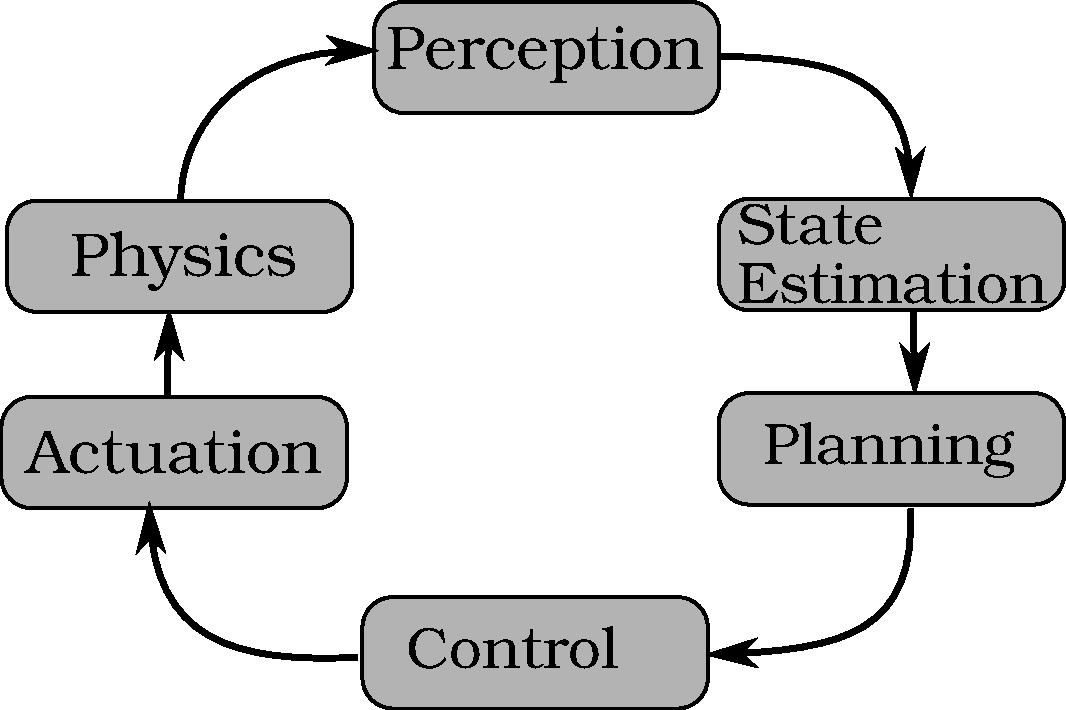
\includegraphics[width=0.6\textwidth]{images/robotics.pdf}

  \end{frame}

  \begin{frame}{Math}

    \begin{align*}
      \arg\min_{T, u(t), q(t)} \quad J(T, u(t), q(t)) \quad \text{s.t.}\\
      q(0) = q_{start} \quad q(T) = q_{goal}\\
      \mathcal{B}(q(t)) \subset \mathcal{W}_{free} \quad \forall t \in [0, T]\\
      \dot q(t) = f(q(t), u(t)) \quad \forall t \in [0, T)
    \end{align*}

  \end{frame}

  \begin{frame}{Video}

    \movie[autostart]{\centering 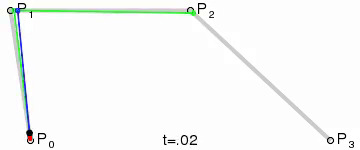
\includegraphics[width=0.5\textwidth]{videos/cubic-bezier.jpg}}{zier.mp4}

  \end{frame}

  \fullscreenvideo{videos/cubic-bezier.jpg}{videos/cubic-bezier.mp4}{https://en.wikipedia.org/wiki/B\%C3\%A9zier\_curve}

  \begin{frame}[fragile]{Source Code}

    \begin{myminted}{python, nobeforeafter, boxsep=0.0mm}
      def Astar(G, d, v_s, v_z, h):
          O = queue()
          while O not empty:
              # smallest f-value
              v = O.pop()
              if v = v_z:
                  return solution
              for n in v.neighbor:
              # ...
    \end{myminted}

  \end{frame}

  \section{Animations}

  \section{Misc}


  \begin{frame}{References}

    Great robotics books \cite{springerHandbook,lavallePlanningBook}

  \end{frame}

  \appendix

  \begin{frame}[standout]
    \inserttitle

    \begin{center}
      \resizebox{!}{0.4\textheight}{?}
    \end{center}

    \begin{columns}
      \begin{column}{0.55\textwidth}
        \begin{itemize}
        \item More Information:\\\url{https://whoenig.github.io}
        \end{itemize}
      \end{column}
      \begin{column}{0.45\textwidth}
        \begin{itemize}
        \item Contact:\\\href{mailto:hoenig@tu-berlin.de}{\texttt{hoenig@tu-berlin.de}}%\\
        \end{itemize}
      \end{column}
    \end{columns}
  \end{frame}

  \begin{frame}[allowframebreaks]{References}
    \printbibliography[heading=none]
  \end{frame}

\end{document}
